
\documentclass{article}
\usepackage[utf8]{inputenc}
\usepackage[spanish.mexico]{babel}
%\title{Dispositivos}
\author{Pablo Vivar Colina}
%\date{Septiembre 2017}

\usepackage{natbib}
\usepackage{graphicx}

%Circuitos
\usepackage{tikz}

\usepackage[american voltages, american currents,siunitx]{circuitikz}

%Diagrama de bloques
%El diagrama de bloques no funciona sin tikz
\usetikzlibrary{shapes.geometric, arrows}

\tikzstyle{startstop} = [rectangle, rounded corners, minimum width=3cm, minimum height=1cm,text centered, draw=black, fill=red!30]
\tikzstyle{io} = [trapezium, trapezium left angle=70, trapezium right angle=110, minimum width=3cm, minimum height=1cm, text centered, draw=black, fill=blue!30]
\tikzstyle{process} = [rectangle, minimum width=3cm, minimum height=1cm, text centered, draw=black, fill=orange!30]
\tikzstyle{decision} = [diamond, minimum width=3cm, minimum height=1cm, text centered, draw=black, fill=green!30]


\tikzstyle{arrow} = [thick,->,>=stealth]
%###MIO###
\tikzstyle{point} = [circle,(0.5cm),minimum with=1cm,draw=black,fill=black!50]




%Circuitos
\usepackage{tikz}

\usepackage[american voltages, american currents,siunitx]{circuitikz}

%Plotting

\usepackage{pgfplots}
\pgfplotsset{width=10cm,compat=1.9} 
 \usepgfplotslibrary{external}
\tikzexternalize 

%#####Fracciones DIAGONALES :B #####

\usepackage{amsmath}
\usepackage{mathtools}

%running fraction with slash - requires math mode.
\newcommand*\rfrac[2]{{}^{#1}\!/_{#2}}


%\maketitle

%\usepackage[top=2cm,bottom=2cm,left=1cm,right=1cm]{geometry}


\begin{titlepage}
     \begin{center}
	
\includegraphics[width=0.09\textwidth]{UNAM}\Large Universidad Nacional Autónoma de México
        	
\includegraphics[width=0.09\textwidth]{FI}\\[1cm]
        \Large Facultad de Ingeniería\\[1cm]
       % \Large División de Ciencias Básicas\\[1cm]
         \Large Laboratorio de Fundamentos de Control(6655)\\[1cm]
         %la clave antes era:4314
         \footnotesize Profesor: Salcedo Ubilla María Leonor Ing.\\[1cm]
        \footnotesize Semestre 2019-1\\[1cm]
        
       

        \Large Práctica No. 1\\[1cm]
        
           

\Large Introdcción MATLAB
        
         %Texto a la derecha
          \begin{flushright}
\footnotesize  Grupo 2\\[0.5cm]
\footnotesize Brigada: 4\\[0.5cm]
\footnotesize Rodrigo Adrián Martínez López\\[0.5cm]
\footnotesize Vivar Colina Pablo\\[0.5cm]
 \end{flushright}
    %Texto a la izquierda
          \begin{flushleft}
        \footnotesize Ciudad Universitaria Agosto de 2018.\\
          \end{flushleft}
         
          
        %\vfill
        %\today
   \end{center}
\end{titlepage}
 %agregar portada

\begin{document}



\tableofcontents  % Write out the Table of Contents

\listoffigures  % Write out the List of Figures


\section{Marco Teórico}

\subsection{Ruido}

La mayoría de las aplicaciones se tiene o considera al ruido r como aditivo, esto es para la señal enviada $s$ se tiene que:\citep{Capitulo1SC}\\

\begin{equation}
    x_r=s+r
\end{equation}

Donde $x_r$ es la señal recibida.\citep{Capitulo1SC}\\

El ruido natural tiende a ser gaussiano, esto es, su densidad es:\citep{Capitulo1SC}

\begin{equation}
    p(n)=\frac{1}{\sqrt{2 \pi \sigma_n}} e^{-\frac{(m-n_m)^2}{2 \sigma_n^2}}
\end{equation}

\begin{figure}[h!]
    \centering
    
   
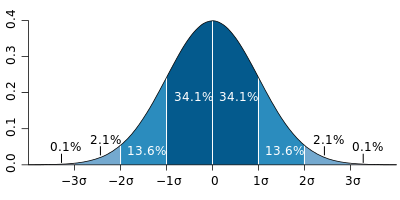
\includegraphics[width=0.6\textwidth]{Imagenes/Standard_deviation_diagram.png}
\caption{ La distribución Normal suele conocerse como la "campana de Gauss".}
    \label{fig:distNorm}
 
\end{figure}


Refiriéndonos a la distribución normal, la cual podemos apreciar en la figura \ref{fig:distNorm} tenemos que:\citep{DistribucionNormal}\\

\begin{itemize}
    \item $\sigma^2$ es la varianza
    \item $n_m$ es la moda
\end{itemize}


El ruido más común es blanco y se define como aquel de densidad de potencia constante.\citep{Capitulo1SC}\\

\begin{equation}
    G_n(f)=\frac{N_0}{2}
\end{equation}

entonces:\\


\begin{equation}
    R_n(\tau)=\frac{N_0}{2} \delta (\tau)
\end{equation}

El ruido térmico es blanco, aditivo y gaussiano, como este ruido esta presente en todos los sistemas de comunicaciones, se utilizan sus características para modelar ruido en comunicaciones.\citep{Capitulo1SC}




\section{Desarrollo}





\subsection{Ruido Blanco en Osciloscopio}

Para el experimento se ajustó el generador de ruido a su amplitud máxima y se conectó al osciloscopio y al analizador de espectros, el oscilograma y lectura del analizador de espectros correspondientes se pueden apreciar en las figuras \ref{fig:RuidoBlanco} y \ref{fig:RuidoBlancoEspectros}.\\

\begin{figure}[h!]
    \centering
    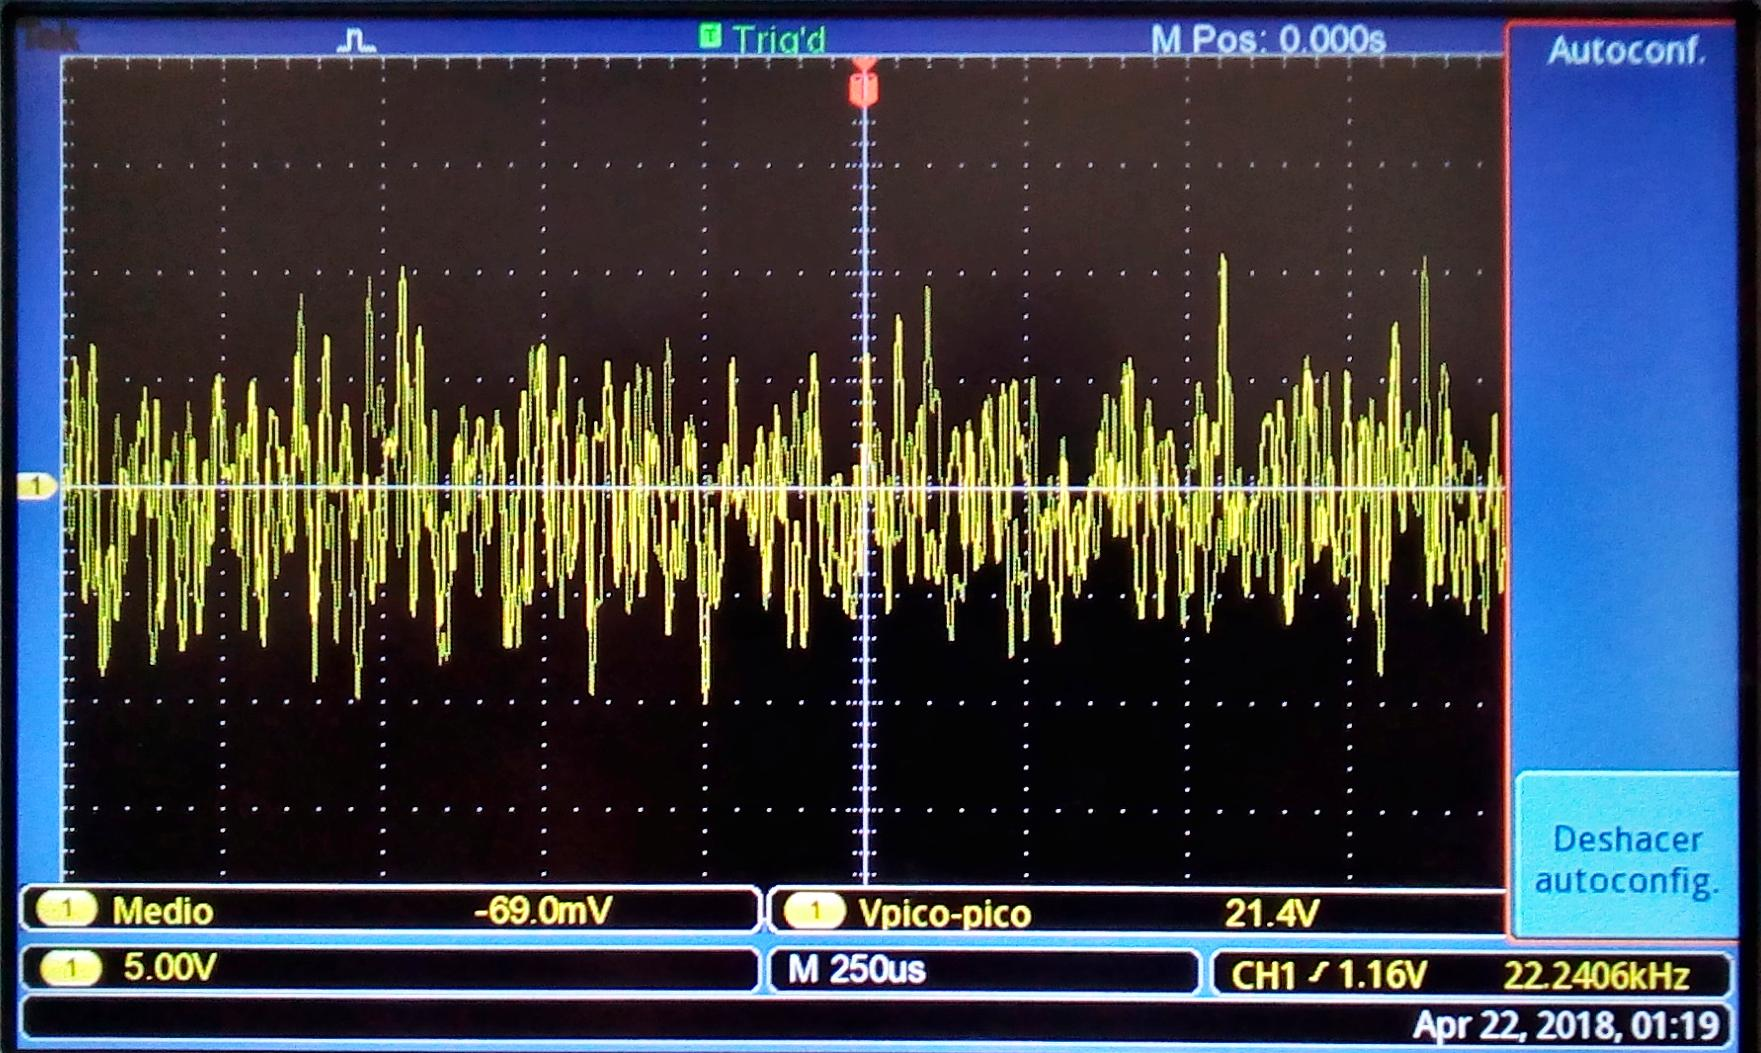
\includegraphics[width=0.7\textwidth]{Imagenes/RuidoBlanco.jpg}
   
    \caption{Ruido Blanco en el osciloscopio}
    \label{fig:RuidoBlanco}
\end{figure}

\begin{figure}[h!]
    \centering
    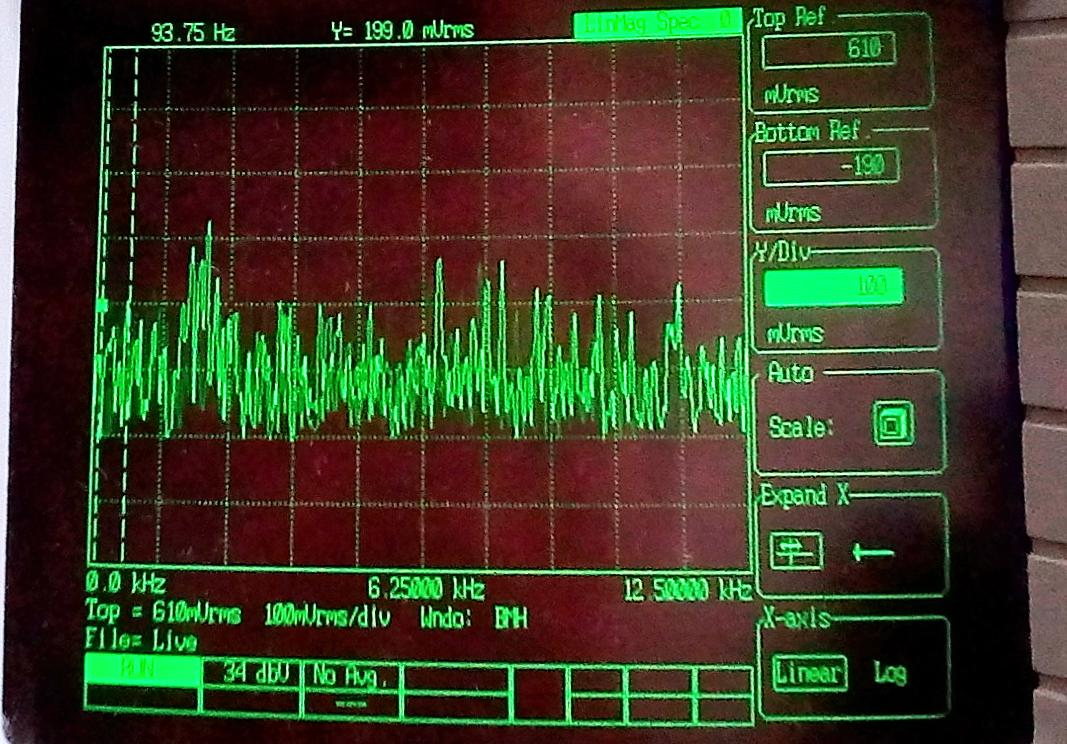
\includegraphics[width=0.7\textwidth]{Imagenes/RuidoBlancoEspectros.jpg}
  
    \caption{Ruido blanco en el analizador de espectros}
    \label{fig:RuidoBlancoEspectros}
\end{figure}


\subection{Ruido Blanco en Bocina}

Posteriormente se conectó al sistema una bocina a la salida del ruido blanco, algunos ejemplos de ruido blanco que se pueden apreciar en la vida cotidiana son:\\

\begin{itemize}
    \item Radio sin señal
    \item Televisión sin señal
    \item agua cayendo aleatoriamientee lluvia, arrollo)
    \item Baleros sin engrasar girando
    \item hojas de lija rasgándose
    \item Semillas o partículas cayendo (palo de lluvia)
\end{itemize}

El ruido blanco en analogía con la luz blanca (que tiene toda la gama de frecuencias de la luz o la mayoría) se dice que tiene toda la gama de frecuencias del sonido, los fenómenos antes listados se asemejan al ruido escuchado en el laboratorio porque están relacionados con partículas que provocan distintos sonido al mismo tiempo, esto se puede explicar debido a la aleatoriedad de sus condiciones. Por ejemplo distintas alturas, distintos tamaños de partículas, entro otros factores que hacen que el ruido generado por cada uno de los elementos que lo conforman sea tan diferente, aunado a que se genera en el mismo tiempo.\\

\subection{Generador de ruido blanco conectado a un filtro}


\begin{figure}[h!]
    \centering
    \begin{tikzpicture}[node distance=4cm]

%startstop-->ROJO
\node (start) [process] {Generador de señales};

\node (GeR) [process,below of=start] {Generador de Ruido};



\node (FPB) [process, right of=start] {Filtro Paso Bajas};



\node (Mult) [process, above of=start] {Multímetro};
%yshift=-0.5cm

\node (Osc) [process, right of=FPB] {Multímetro};
%yshift=-0.5cm



%Línea inicio a filtro paso bajas
\draw [arrow] (start) -- (FPB);


%Línea de generador de ruido a filtro paso bajas 
\draw [arrow] (GeR) -|(FPB);



\draw [arrow] (Mult) -|(FPB);

\draw [arrow] (FPB) --(Osc);


\end{tikzpicture}
    \caption{Sistema con generador de ruido blanco ($f=[1kHz],v=v_{ruido}$}
    \label{fig:sistRuidoBlanco}
\end{figure}


Para el experimento siguiente se conectó el generador de funciones con una función senoidal de 1 [kHz] en paralelo con el generador de ruido blanco para ésto teniendo el equipo previamente conectado se midió con el multímetro el voltaje (RMS) del generador del ruido blanco y se ingresó el mismo valor en el generador de funciones, el sistema de éste experimento se puede apreciar en el gráfico \ref{fig:DiagramaBloques} y el oscilograma del osciloscopio y el espectro del experimento se pueden apreciar en  las figuras: \ref{fig:ruidoSenoFiltro} y \ref{fig:ruidoSenoEspectros}.\\

%\begin{figure}[h!]
 %   \centering
  %  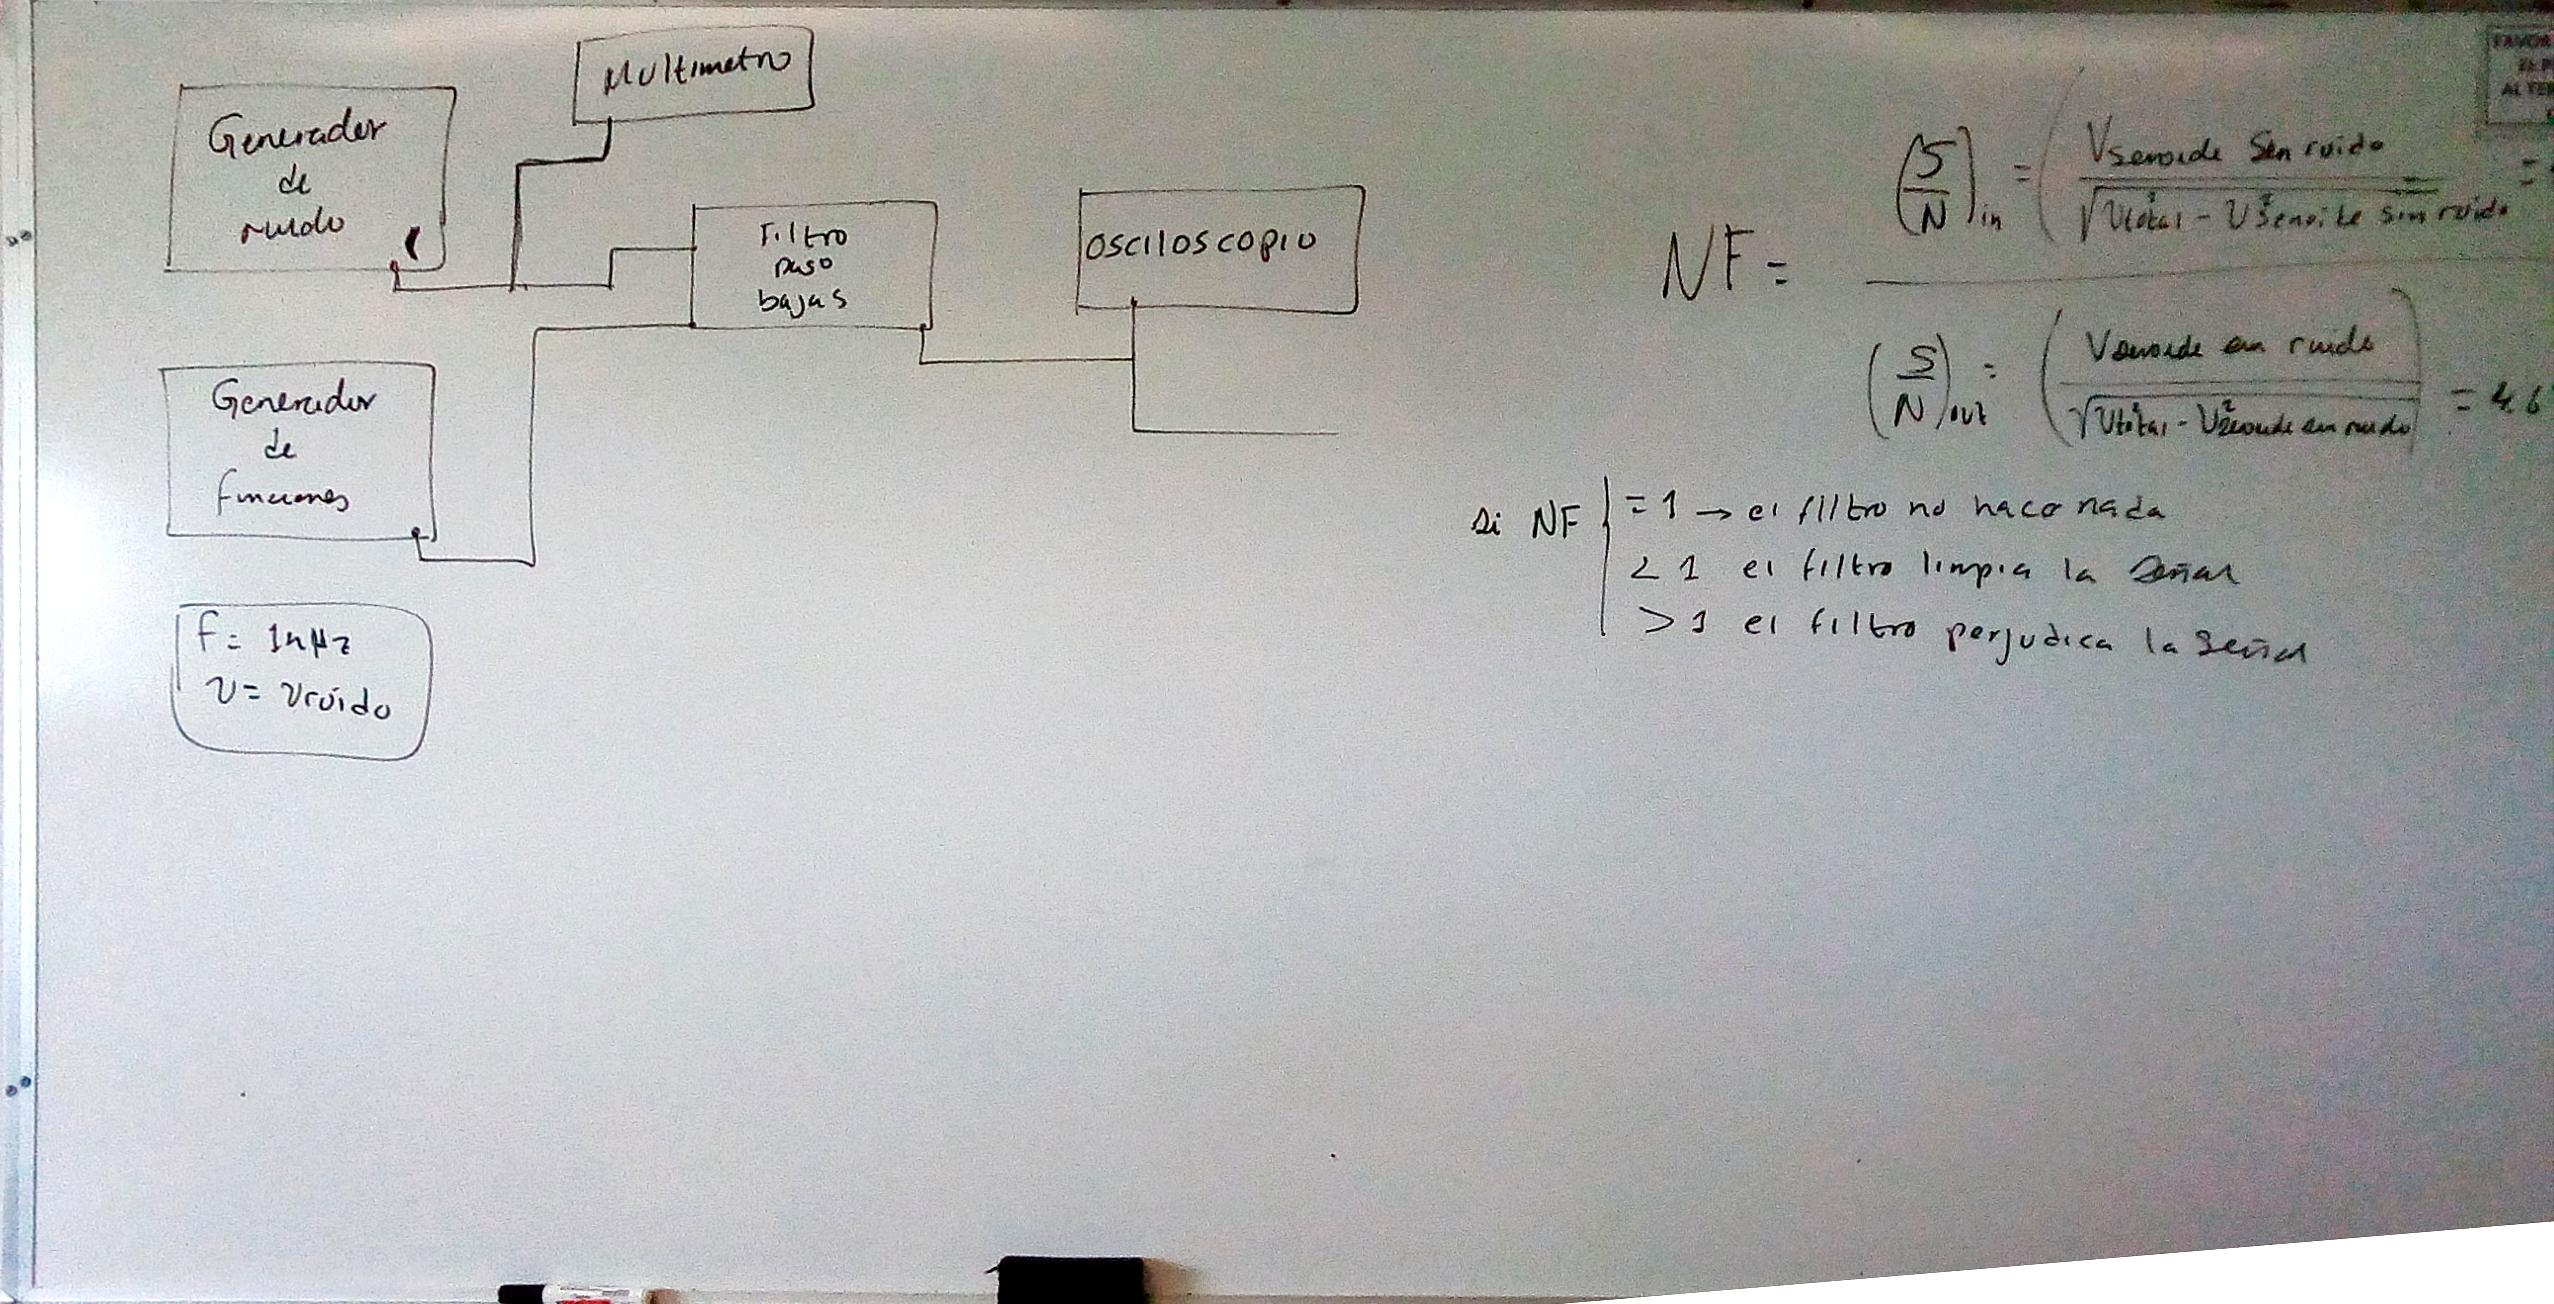
\includegraphics[width=0.7\textwidth]{Imagenes/DiagramaBloques.jpg}
   
   % \caption{Diagrama de Bloques}
    %\label{fig:DiagramaBloques}
%\end{figure}

%\begin{figure}[h!]
 %   \centering
  %  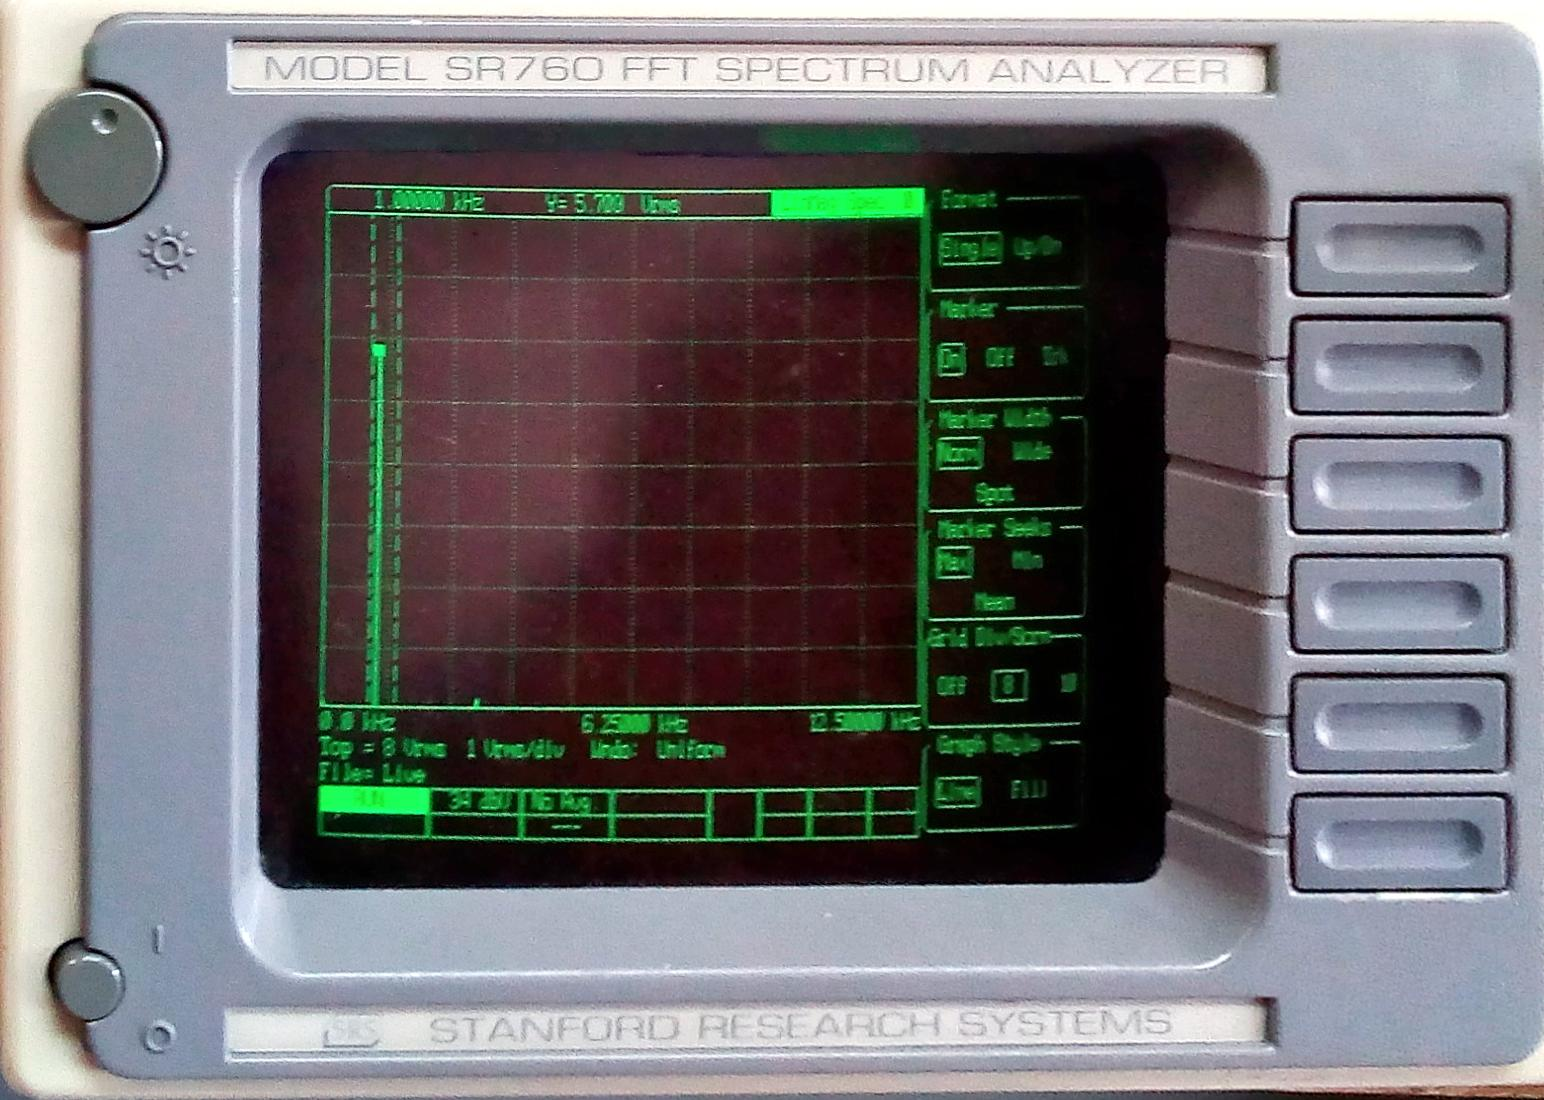
\includegraphics[width=0.7\textwidth]{Imagenes/EspectroRuidoSenoFiltro.jpg}
  
   % \caption{}
%    \label{fig:EspectroRuidoSenoFiltro}
%\end{figure}

%\begin{figure}[h!]
    %\centering
   % 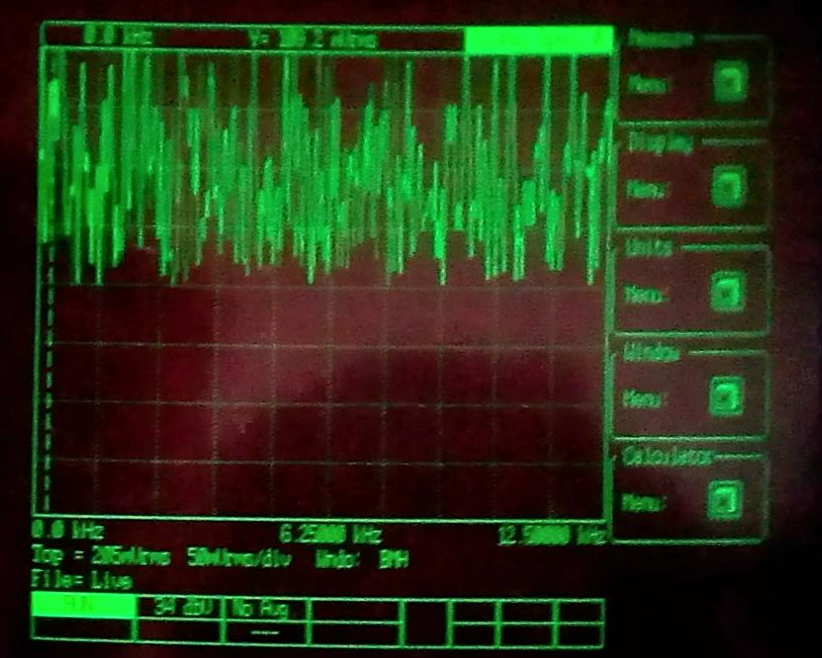
\includegraphics[width=0.7\textwidth]{Imagenes/RuidoEspectrosArr.png.jpg}
   
  %  \caption{Diagrama de Bloques}
 %   \label{fig:Ruido Espectros Arreglos}
%\end{figure}

\begin{figure}[h!]
    \centering
    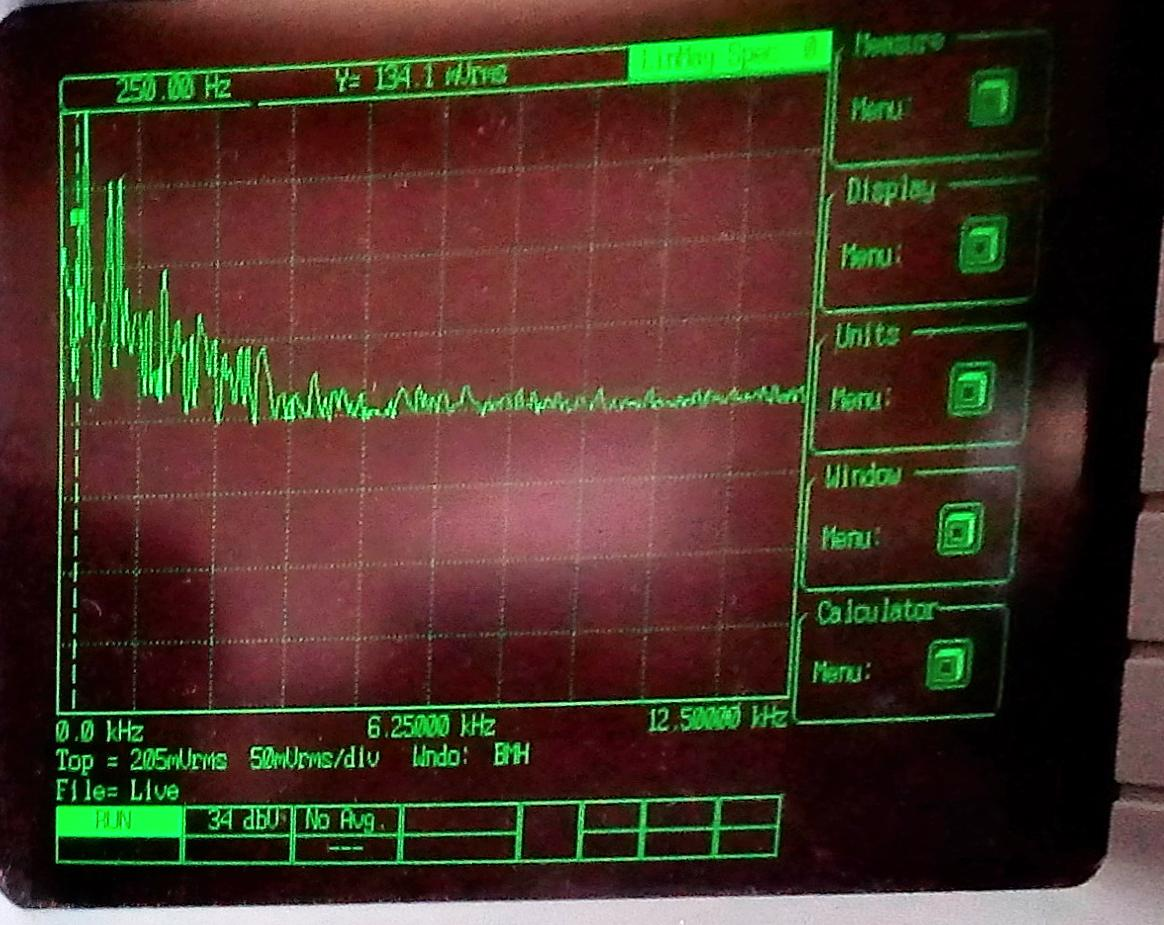
\includegraphics[width=0.7\textwidth]{Imagenes/RuidoSenoEspectros.jpg}
    
    \caption{Señal de 1[kHz] con generador de ruido Blanco}
    \label{fig:ruidoSenoEspectros}
\end{figure}

\begin{figure}[h!]
    \centering
    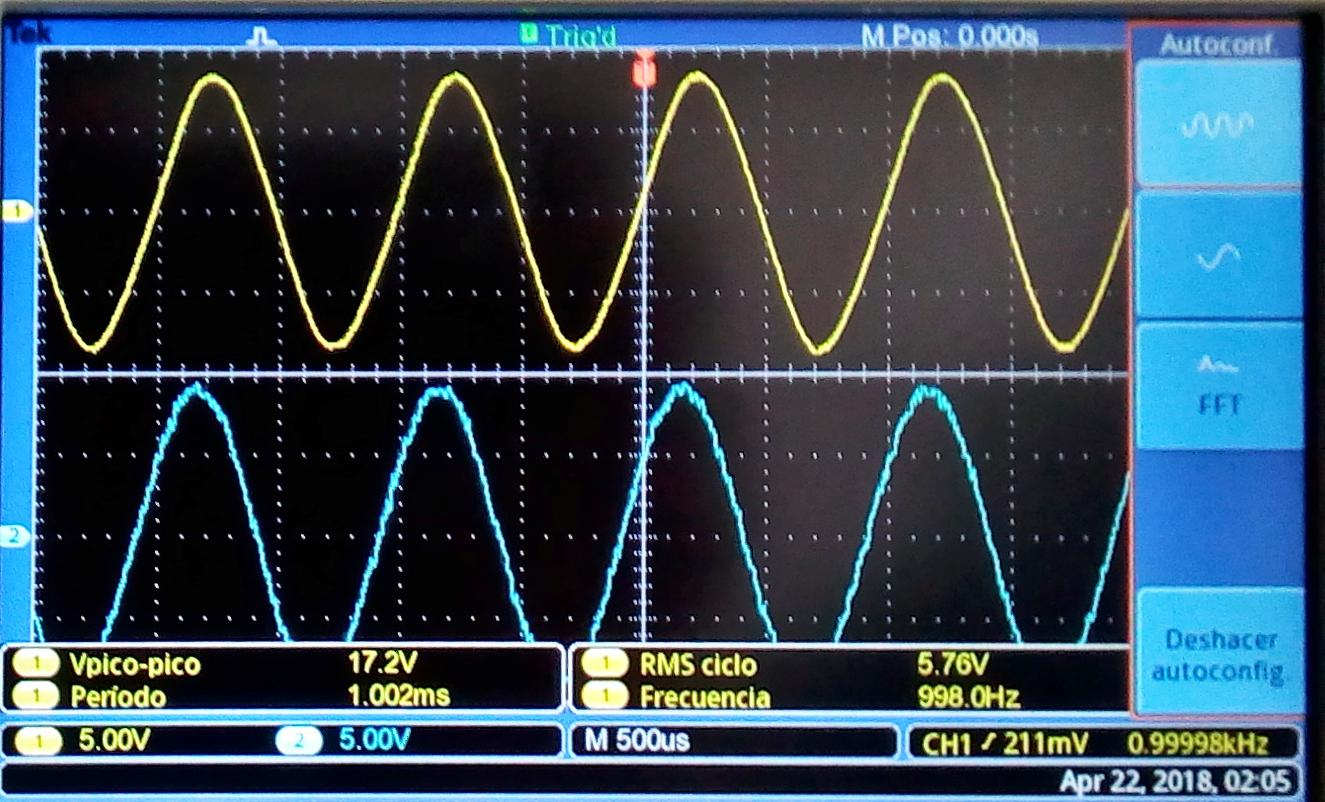
\includegraphics[width=0.7\textwidth]{Imagenes/RuidoSenoFiltro.jpg}
   
    \caption{Espectro a la salida del sistema mostrado en \ref{fig:DiagramaBloques}}
    \label{fig:ruidoSenoFiltro}
\end{figure}

La relación señal ruido se puede obtener mediante la expresión:\\

\begin{equation}
    \frac{S}{N}=\frac{V_{senoSinRuido}}{\sqrt{V_{total}^2-V_{senoSinRuido}^2}}
\end{equation}

Para éste experimento se determinarosn éstas relaciones en la entrada y en la salida del sistema, los voltajes a ocupar fueron los siguientes:\\

\begin{itemize}
    \item $V_{totalEntrada}=2.95[V]$
    \item $V_{totalSalida}=2.64[V]$
    \item $V_{senoEntrada}=2.81[V]$
    \item $V_{senoSalida}=2.5[V]$
\end{itemize}

Por lo que la relaciones sonido ruido obtenidas en la entrada y en la salida fueron las siguientes.\\

\begin{itemize}
    \item A la entrada: 3.12
    \item A la salida: 2.94
\end{itemize}

\section{Conclusiones Pablo Vivar Colina}

Se pudo apreciar como puede el ruido afectar una señal, se conoce que el ruido puede generarse por distintos motivos (líneas de transmisión, efectos electromagnéticos, etc.) y es necesario tener éste fenómeno presente para que la información pueda ser reconocible por el receptor, y es por eso que se necesitan diseñar filtros que nos ayuden a recuperar la información lo más parecida posible a lo que el transmisor ha enviado.

\section{Comentarios Pablo Vivar Colina}

El ruido es algo que se busca suprimir en una señal, sin embargo el generador de ruido blanco puede ser una buena aproximación del ruido que se presentará en una línea de comunicaciones, y es útil para poder diseñar filtros que nos ayuden a suprimir éste tipo de imperfecciones en los sistemas de comunicación.

%.\\[100cm]
\bibliographystyle{plain}
\bibliography{Referencias.bib}

\end{document}
